%&pdflatex
\documentclass{standalone}
\usepackage{tikz}
\usetikzlibrary{arrows}
\usetikzlibrary{shapes}

\begin{document}

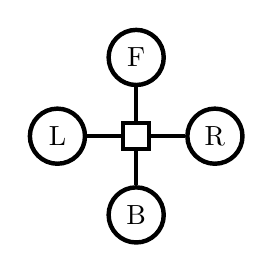
\begin{tikzpicture}
    \node [draw, ultra thick, regular polygon,regular polygon sides=4] (body) {};
    \node [draw, ultra thick, circle, right of=body, minimum size=0.7cm] (right) {R};
    \node [draw, ultra thick, circle, left of=body, minimum size=0.7cm] (left) {L};
    \node [draw, ultra thick, circle, below of=body, minimum size=0.7cm] (back) {B};
    \node [draw, ultra thick, circle, above of=body, minimum size=0.7cm] (front) {F};
    
    \draw [ultra thick] (body) -- (right);
    \draw [ultra thick] (body) -- (left);
    \draw [ultra thick] (body) -- (back);
    \draw [ultra thick] (body) -- (front);
    
\end{tikzpicture}

\end{document}



